%iffalse
\let\negmedspace\undefined
\let\negthickspace\undefined
\documentclass[journal,12pt,onecolumn]{IEEEtran}
\usepackage[version=4]{mhchem}
\usepackage{chemformula} % for \ch if needed
\usepackage{chemfig}
\usepackage{chemmacros}
\chemsetup{modules = reactions} % Enables reaction arrows
\usepackage{graphicx}
\graphicspath{ {./images/} }
\usepackage{geometry}
\usepackage{lastpage}
\usepackage{cite}
\usepackage{amsmath,amssymb,amsfonts,amsthm}
\usepackage{enumitem,multicol}
\usepackage{algorithmic}
\usepackage{graphicx}
\usepackage{textcomp}
\usepackage{xcolor}
\usepackage{txfonts}
\usepackage{listings}
\usepackage{enumitem}
\usepackage{mathtools}
\usepackage{gensymb}
\usepackage{comment}
\usepackage[breaklinks=true]{hyperref}
\usepackage{tkz-euclide} 
\usepackage{listings}
\usepackage{gvv}                                        
%\def\inputGnumericTable{}                                 
\usepackage[latin1]{inputenc}                                
\usepackage{color}                                            
\usepackage{array}                                            
\usepackage{longtable}                                       
\usepackage{calc}                                             
\usepackage{multirow}                                         
\usepackage{hhline}                                           
\usepackage{ifthen}                                           
\usepackage{lscape}
\usepackage{tabularx}
\usepackage{array}
\usepackage{float}


\newtheorem{theorem}{Theorem}[section]
\newtheorem{problem}{Problem}
\newtheorem{proposition}{Proposition}[section]
\newtheorem{lemma}{Lemma}[section]
\newtheorem{corollary}[theorem]{Corollary}
\newtheorem{example}{Example}[section]
\newtheorem{definition}[problem]{Definition}
\newcommand{\BEQA}{\begin{eqnarray}}
\newcommand{\EEQA}{\end{eqnarray}}
\newcommand{\define}{\stackrel{\triangle}{=}}
\theoremstyle{remark}

\geometry{margin=1 in}



\setlength{\headheight}{14pt}
\setlength{\headsep}{5pt}
\setlength{\footskip}{20pt}
\begin{document}
1-5 carry one mark each
\begin{enumerate}
    \item Choose the appropriate word/phrase, out of the four options given below, to complete the following sentence:\\
Apparent lifelessness \rule{2cm}{0.15mm} dormant life.
\hfill{GATE 2015 PI}

\begin{multicols}{2}
\begin{enumerate}
    \item harbours
    \item leads to
    \item supports
    \item affects
\end{enumerate}
\end{multicols}

\item Fill in the blank with the correct idiom/phrase.\\
That boy from the town was a \rule{2cm}{0.15mm} in the sleepy village.
\hfill{GATE 2015 PI}

\begin{multicols}{2}
\begin{enumerate}
    \item dog out of herd
    \item sheep from the heap
    \item fish out of water
    \item bird from the flock
\end{enumerate}
\end{multicols}
\item Choose the statement where underlined word is used correctly.
\hfill{GATE 2015 PI}

\begin{multicols}{2}
\begin{enumerate}
    \item When the teacher eludes to different authors, he is being elusive.
    \item When the thief keeps eluding the police, he is being elusive
    \item Matters that are difficult to understand, identify or remember are \textit{allusive}.
    \item Mirages can be allusive, but a better way to express them is illusory.
\end{enumerate}
\end{multicols}

\item Tanya is older than Eric.\\
Cliff is older than Tanya.\\
Eric is older than Cliff.

If the first two statements are true, then the third statement is:
\hfill{GATE 2015 PI}

\begin{multicols}{2}
\begin{enumerate}
    \item True
    \item False
    \item Uncertain
    \item Data insufficient
\end{enumerate}
\end{multicols}
\item Five teams have to compete in a league, with every team playing every other team exactly once, before going to the next round. How many matches will have to be held to complete the league round of matches?
\hfill{GATE 2015 PI}

\begin{multicols}{2}
\begin{enumerate}
    \item 20
    \item 10
    \item 8
    \item 5
\end{enumerate}
\end{multicols}
6-10 carry two marks each
\item Select the appropriate option in place of underlined part of the sentence.\\
\textit{Increased productivity necessary} reflects greater efforts made by the employees.
\hfill{GATE 2015 PI}

\begin{multicols}{2}
\begin{enumerate}
    \item Increase in productivity necessary
    \item Increase productivity is necessary
    \item Increase in productivity necessarily
    \item No improvement required
\end{enumerate}
\end{multicols}
\item Given below are two statements followed by two conclusions. Assuming these statements to be true, decide which one logically follows.

Statements:
\begin{enumerate}
    \item No manager is a leader.
    \item All leaders are executives.
\end{enumerate}

Conclusions:
\begin{enumerate}
    \item No manager is an executive.
    \item No executive is a manager.
\end{enumerate}

\hfill{GATE 2015 PI}

\begin{multicols}{2}
\begin{enumerate}
    \item Only conclusion I follows.
    \item Only conclusion II follows.
    \item Neither conclusion I nor II follows.
    \item Both conclusions I and II follow.
\end{enumerate}
\end{multicols}
\item In the given figure angle Q is a right angle, PS:QS = 3:1, RT:QT = 5:2 and PU:UR = 1:1. If area of triangle QTS is 20 cm$^2$, then the area of triangle PQR in cm$^2$ is \underline{\hspace{3cm}}.

\begin{figure}[H]
    \centering
    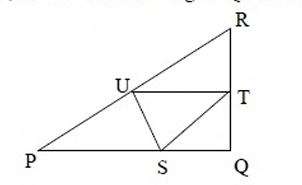
\includegraphics[width=0.5\linewidth]{figs/Q.8.png}
    \caption{fig1}
    \label{fig:figs/Q.8.png}
\end{figure}
\hfill{GATE 2015 PI}

\item Right triangle PQR is to be constructed in the xy-plane so that the right angle is at P and line PR is parallel to the x-axis. The x and y coordinates of P, Q, and R are to be integers that satisfy the inequalities: $-4 \leq x \leq 5$ and $6 \leq y \leq 16$. How many different triangles could be constructed with these properties?
\hfill{GATE 2015 PI}

\begin{multicols}{2}
\begin{enumerate}
    \item 110
    \item 1,100
    \item 9,900
    \item 10,000
\end{enumerate}
\end{multicols}

\item A coin is tossed thrice. Let $X$ be the event that head occurs in each of the first two tosses. Let $Y$ be the event that a tail occurs on the third toss. Let $Z$ be the event that two tails occur in three tosses. Based on the above information, which one of the following statements is TRUE?
\hfill{GATE 2015 PI}

\begin{multicols}{2}
\begin{enumerate}
    \item $X$ and $Y$ are not independent
    \item $Y$ and $Z$ are dependent
    \item $Y$ and $Z$ are independent
    \item $X$ and $Z$ are independent
\end{enumerate}
\end{multicols}
11-35 carry one mark each
\item In numerical integration using Simpson's rule, the approximating function in the interval is a
\hfill{GATE 2015 PI}

\begin{multicols}{2}
\begin{enumerate}
    \item constant
    \item straight line
    \item cubic B-Spline
    \item parabola
\end{enumerate}
\end{multicols}

\item If a constant force $\vec{f}$ applied on an object $P$, displaces it by a distance $\vec{d}$, inclined at an angle $\theta$ to the direction of force $\vec{f}$, then the work done by the force $\vec{f}$ is
\hfill{GATE 2015 PI}

\begin{multicols}{2}
\begin{enumerate}
    \item $\mathrm{div}(\vec{f} \times \vec{d})$
    \item $\left| \vec{f} \times (\mathrm{curl} \vec{d}) \right|$
    \item $\left| \vec{f} \times \vec{d} \right|$
    \item $\vec{f} \cdot \vec{d}$
\end{enumerate}
\end{multicols}

\item A product is an assembly of 5 different components. The product can be sequentially assembled in two possible ways. If the 5 components are placed in a box and these are drawn at random from the box, then the probability of getting a correct sequence is


\hfill{GATE 2015 PI}
\begin{enumerate}
    \item $\dfrac{2}{5!}$
    \item $\dfrac{2}{5}$
    \item $\dfrac{2}{(5-2)!}$
    \item $\dfrac{2}{(5-3)!}$
\end{enumerate}





\item The function $f(x) = x^2 = x + x + x + \ldots$ $x$ times, is defined
\hfill{GATE 2015 PI}

\begin{enumerate}
    \item at all real values of $x$
    \item only at positive integer values of $x$
    \item only at negative integer values of $x$
    \item only at rational values of $x$
\end{enumerate}
\item The room-temperature stress ($\sigma$)-strain ($\varepsilon$) curves of four materials P, Q, R, and S are shown in the figure below. The material that behaves as a rigid perfectly plastic material is

\begin{enumerate}
    \item P
    \item Q
    \item R
    \item S
\end{enumerate}

\hfill{GATE 2015 PI}

\item The true stress at fracture of a tensile tested specimen, having an initial diameter of 13 mm, is 700 MPa. If the diameter of specimen at fracture is 10 mm, then the engineering stress, in MPa, at fracture is \underline{\hspace{3cm}}.

\hfill{GATE 2015 PI}
\item If the principal stress values are 120 MPa, $-50$ MPa and 10 MPa in a given state of stress, then maximum shear stress in the material, in MPa, is \underline{\hspace{3cm}}.

\hfill{GATE 2015 PI}

\item Match the items in the first column to their functions in the second column.

\begin{tabbing}
\hspace{2cm} \= \kill
P. Sprue         \> 1. regulates flow of molten metal into mould cavity \\
Q. Riser         \> 2. feeds molten metal from pouring basin to gate \\
R. Gate          \> 3. acts as a reservoir for molten metal \\
S. Pouring basin   \> 4. supplies molten metal to compensate
forliquid shrinkage   \\
\end{tabbing}

\hfill{GATE 2015 PI}

\begin{enumerate}
    \item (A) P-1, Q-2, R-3, S-4
    \item (B) P-2, Q-4, R-1, S-3
    \item (C) P-4, Q-2, R-1, S-3
    \item (D) P-2, Q-4, R-3, S-1
\end{enumerate}
\item In rolling of a flat strip, the relative velocity of strip with respect to the roller is

\begin{enumerate}
    \item positive at entry plane, negative at exit plane
    \item negative at entry plane, positive at exit plane
    \item positive throughout from entry to exit plane
    \item negative throughout from entry to exit plane
\end{enumerate}

\hfill{GATE 2015 PI}



\item The maximum reduction per pass during wire drawing of an aluminum alloy ignoring friction and redundant work is 77\%. The strain hardening exponent of the material is \underline{\hspace{3cm}}.

\hfill{GATE 2015 PI}

\item Built-up edge formation decreases under the conditions listed below \textbf{EXCEPT}

\begin{enumerate}
    \item at low cutting speeds
    \item using large positive rake angle
    \item with sharper tool
    \item using cutting fluid
\end{enumerate}

\hfill{GATE 2015 PI}
\item During turning of mild steel work material, the maximum temperature is observed at 

\hfill{GATE 2015 PI}
\begin{enumerate}
\begin{multicols}{2}
\item primary deformation zone
\item tool and chip interface
\item tool-flank and work interface
\item machined sub-surface
\end{multicols}
\end{enumerate}

\item Which one of the following statements related to grinding process is \textbf{INCORRECT}? 

\hfill{GATE 2015 PI}
\begin{enumerate}
\begin{multicols}{2}
\item Grinding wheels made of finer abrasive grains produce better surface finish.
\item Abrasive grains tend to fracture frequently during the grinding process.
\item Specific energy in grinding is higher than that in turning.
\item Cutting speed in grinding process is much lower than that in face milling.
\end{multicols}
\end{enumerate}

\item For an assembly made of $n$ components, the dimensions on each component $i$ follow a normal distribution and have tolerance $T_{i}$. Overall dimension of the assembly is $L_{a}$ with tolerance $T_{a}$. The relationship between $T_{a}$ and $T_{i}$ is
\hfill{GATE 2015 PI}
\begin{enumerate}
\begin{multicols}{2}
\item $T_{a} = L_{a} \sqrt{\sum_{i=1}^{n}\dfrac{T_{i}^2}{L_{a}^2}}$
\item $T_{a} = \sqrt{\sum_{i=1}^{n} T_{i}^2}$
\item $T_{a} = L_{a} + \sqrt{\sum_{i=1}^{n} T_{i}^2}$
\item $T_{a} = L_{a} + \sum_{i=1}^{n} T_{i}^2$
\end{multicols}
\end{enumerate}
\item Which of the following \textbf{DO NOT} influence the material removal rate in Electrical Discharge Machining process?
\begin{enumerate}
    \item Hardness of work piece material
    \item Melting temperature of work piece material
    \item Hardness of tool material
    \item Discharge current and frequency
\end{enumerate}
\begin{enumerate}
    \item (i) and (ii)
    \item (i) and (iii)
    \item (iii) and (iv)
    \item (i), (ii) and (iii)
\end{enumerate}


\item In Computer Aided Process Planning, determination of process sequence for manufacture of any part design without predefined standard plans is known as
\begin{enumerate}
    \item variant type process planning
    \item retrieval type process planning
    \item generative type process planning
    \item group technology based process planning
\end{enumerate}


\item The angle of a twist drill that determines its rake angle is
\begin{enumerate}
    \item lip relief angle
    \item chisel edge angle
    \item helix angle
    \item point angle
\end{enumerate}
\item A line balancing problem is solved in the context of \hfill{GATE 2015 PI}
\begin{enumerate}
    \item process layout
    \item fixed position layout
    \item product layout
    \item production schedule
\end{enumerate}

\item Solution to the balanced assignment problem is binary due to \hfill{GATE 2015 PI}
\begin{enumerate}
    \item linear formulation
    \item non-empty feasible region
    \item approximation algorithms
    \item uni-modularity property
\end{enumerate}


\item Material Requirements Planning \textbf{DOES NOT} include \hfill{GATE 2015 PI}
\begin{enumerate}
    \item material price
    \item bill of material
    \item inventory level
    \item production schedule
\end{enumerate}

\item Ishikawa diagram represents
\begin{enumerate}
    \item different types of quality defects
    \item quantitative relation between the extent of defect and a process parameter
    \item relation between defects and their causes
    \item prioritized quality defects
\end{enumerate}

\item As per the principles of motion economy, which one of the following is \textbf{NOT} a pivot for a classified movement of human body? \hfill{GATE 2015 PI}
\begin{enumerate}
    \item Knee
    \item Elbow
    \item Torso
    \item Wrist
\end{enumerate}

\item For air travel over a distance of 500 km, the ticket price is Rs. 4000. The comfort of the air travel can be monetized at Rs. 3000, and the monetary value of time saved because of air travel is Rs. 3000. The value of air travel is \underline{\hspace{2cm}}.
\item Which one of the following is NOT in the scope of Enterprise Resource Planning (ERP) system? 

\hfill{GATE 2015 PI}
\begin{enumerate}
    \item General ledger entries
    \item Materials management system
    \item Order management system
    \item Employee promotion policy
\end{enumerate}

\item If standard production is 20 units, a worker's actual output is 18 units, piece rate is Rs. 500 per unit, and over-achievement rate is Rs. 750 per unit, then the wage paid to the worker, in Rs., as per Taylor's differential price rate wage incentive plan, is \underline{\hspace{2cm}}. \hfill{GATE 2015 PI}

\item The solution to $6yy' - 25x = 0$ represents a \hfill{GATE 2015 PI}
\begin{enumerate}
    \item family of circles
    \item family of ellipses
    \item family of parabolas
    \item family of hyperbolas
\end{enumerate}
\item The solution to $x^2 y'' + xy' - y = 0$ is \hfill{GATE 2015 PI}
\begin{enumerate}
    \item $y = c_1 x^2 + c_2 x^{-3}$
    \item $y = c_1 + c_2 x^{-2}$
    \item $y = c_1 x + \frac{c_2}{x}$
    \item $y = c_1 x + c_2 x^4$
\end{enumerate}

\item Match the linear transformation matrices listed in the first column to their interpretations in the second column. \hfill{GATE 2015 PI}

\begin{tabular}{|c|c|c|}
\hline
\textbf{Matrix} & & \textbf{Interpretation} \\
\hline
P.\ $\begin{bmatrix} 1 & 0 \\ 0 & 0 \end{bmatrix}$ &  & 1. Stretch in the y-axis \\
Q.\ $\begin{bmatrix} 0 & 0 \\ 0 & 1 \end{bmatrix}$ &  & 2. Uniform stretch in x and y-axes \\
R.\ $\begin{bmatrix} 1 & 0 \\ 0 & 3 \end{bmatrix}$ &  & 3. Projection in x-axis \\
S.\ $\begin{bmatrix} 4 & 0 \\ 0 & 4 \end{bmatrix}$ &  & 4. Projection in y-axis \\
\hline
\end{tabular}

\begin{enumerate}
    \item P-1, Q-2, R-3, S-4
    \item P-2, Q-3, R-4, S-1
    \item P-3, Q-4, R-1, S-2
    \item P-4, Q-1, R-2, S-3
\end{enumerate}

\item The value of $\lim\limits_{(x, y) \to (0, 0)} \frac{x^2 - xy}{\sqrt{x} - \sqrt{y}}$ is \hfill{GATE 2015 PI}
\begin{enumerate}
    \item 0
    \item $\dfrac{1}{2}$
    \item 1
    \item $\infty$
\end{enumerate}

\item The curve $y = x^4$ is \hfill{GATE 2015 PI}
\begin{enumerate}
    \item concave up for all values of $x$
    \item concave down for all values of $x$
    \item concave up only for positive values of $x$
    \item concave up only for negative values of $x$
\end{enumerate}

\item A metallic bar of uniform cross-section with specific weight of $100$ kN/m$^3$ is hung vertically down. The length and Young's modulus of the bar are $100$ m and $200$ GPa, respectively. The elongation of the bar, in mm, due to its own weight is \underline{\hspace{2cm}}. \hfill{GATE 2015 PI}

\item The bending moment, in Nm, at point R is \underline{\hspace{2cm}}. \hfill{GATE 2015 PI}

\item In an off-set slider crank mechanism, shown in figure, the crank is rotated at a constant speed of 150 rpm. The value of the angle $\theta$ shown in the figure is $20^\circ$. What is the ratio of forward to return stroke time? Can this mechanism be used in an application involving quick return? \hfill{GATE 2015 PI}
\begin{enumerate}
    \item 3.33, No
    \item 0.73, Yes
    \item 1.25, Yes
    \item 0.73, No
\end{enumerate}

\item In a 1 m thick wall, the temperature distribution at a given instant is $T(x) = c_0 + c_1 x + c_2 x^2$ where $T$ is in $^\circ$C and $x$ is in m. The constants are: $c_0 = 800~^\circ$C, $c_1 = -250~^\circ$C/m and $c_2 = -40~^\circ$C/m$^2$. The thermal conductivity of the wall is $50$ W/mK and wall area is $5$ m$^2$. If there is a heat source generating uniform volumetric heating at the rate of $500$ W/m$^3$ inside the wall, then the rate of change of energy storage in the wall, in kW, is \underline{\hspace{2cm}}. \hfill{GATE 2015 PI}

\item In a vertical piston-cylinder arrangement the force applied to the piston pushes water through a nozzle. The water flows out from the nozzle and reaches the top of its trajectory. The kinetic and pressure energies at points (1), (2) and (3), respectively, are \hfill{GATE 2015 PI}
\begin{enumerate}
    \item (small and large), (large and zero) and (zero and zero)
    \item (small and zero), (large and large) and (small and zero)
    \item (large and zero), (zero and large) and (large and zero)
    \item (large and small), (small and zero) and (small and large)
\end{enumerate}
\item Consider a glass-fiber reinforced polymer material. The stress-strain curves of the fiber, matrix and composite are plotted. Which one of the following statements is \textbf{TRUE}? \hfill{GATE 2015 PI}
\begin{enumerate}
    \item Curve P represents the composite, Curve Q the matrix and Curve R the fiber.
    \item Curve Q represents the composite, Curve R the matrix and Curve P the fiber.
    \item Curve R represents the composite, Curve P the matrix and Curve Q the fiber.
    \item Curve P represents the composite, Curve R the matrix and Curve Q the fiber.
\end{enumerate}
\item A mould for injection moulding is designed for polymer P having shrinkage of 0.010 mm/mm. A critical dimension needed in the moulded part is 35 mm. If the same mould is now used to make a similar part but made of a different polymer Q with shrinkage of 0.025 mm/mm, then the critical dimension in the moulded part made of polymer Q, in mm, is \underline{\hspace{2cm}}. \hfill{GATE 2015 PI}

\item Open die forging of a cylinder made of a rigid perfectly plastic material with yield strength of 200 MPa having a height of 25 mm and diameter of 25 mm is being carried out. The cylinder is subjected to a true compressive strain of 3.6 during the process. Assuming frictionless and homogeneous deformation, the energy expended, in kJ, is \underline{\hspace{2cm}}. \hfill{GATE 2015 PI}

\item In drilling operation, a twist-drill of 30 mm diameter with point angle of 118 degrees is used. If the CNC command issued to execute the drilling operation is G90 G01 Z?? F20. The datum is defined on the top surface of the work material and the approach distance is 3 mm. Then, to achieve a cylindrical hole depth of 40 mm, the Z coordinate to be provided in the CNC command, in mm, is \underline{\hspace{2cm}}. \hfill{GATE 2015 PI}
\item In an orthogonal machining experiment carried out using a cutting tool with zero degree rake angle, the measured cutting force was 1700 N. If the friction angle at the rake face-chip interface is $26^\circ$, then the thrust force value, in N, is \underline{\hspace{2cm}}. \hfill{GATE 2015 PI}

\item In a slab milling operation, a cutter of 75 mm diameter with sufficient width is used to remove 5 mm thick material from a 200 mm long part in a single pass. The minimum length of travel, in mm, for the cutter to engage and completely cut the part surface is \underline{\hspace{2cm}}. \hfill{GATE 2015 PI}

\item In a metal casting process, molten copper alloy is poured into a sand mould. The level of molten metal in the pouring basin is at a height of 300 mm from the runner having diameter of 10 mm. If the density and melting temperature of molten copper alloy are 9000 kg/m$^3$ and 1000$^\circ$C, respectively, then the rate of flow of molten metal into the mould neglecting friction and other losses, in cm$^3$/s, is \underline{\hspace{2cm}}. \hfill{GATE 2015 PI}

\item Two aluminum alloy plates each 10 mm thick and 1 m long are welded without crowning by multi-pass tungsten inert gas butt welding. The joint configuration is V-type with 60$^\circ$ angle and root gap is maintained at 5 mm. If electrode of 5 mm diameter with 500 mm length is used for welding, then the number of electrodes required is \hfill{GATE 2015 PI}
\begin{enumerate}
\begin{multicols}{2}
    

    \item 7
    \item 9
    \item 11
    \item 13
    \end{multicols}
\end{enumerate}

\item A surface is prepared specially for an application with the profile as shown. The theoretical $R_a$ value for this surface, in $\mu$m, is \underline{\hspace{2cm}}
\begin{figure}[H]
    \centering
    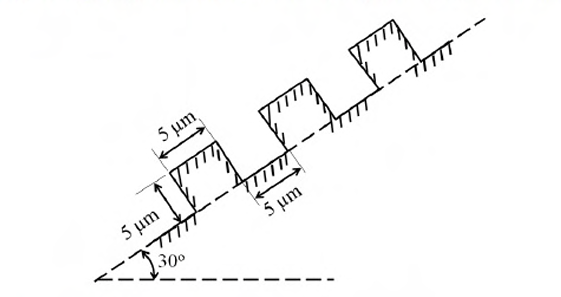
\includegraphics[width=0.5\linewidth]{figs/Q.54.png}
    \caption{fig2}
    \label{fig:figs/Q.54.png}
\end{figure}





\hfill{GATE 2015 PI}
\item During the measurement of internal taper of a part using standard balls of diameter 15 mm and 20 mm, the large ball is found to protrude by 5 mm ($h_1$) and the top of small ball is found to be 35 mm ($h_2$) below the top face of the gauge. The taper angle, in degree, is \underline{\hspace{2cm}}. \hfill{GATE 2015 PI}

\item In a Flexible Manufacturing System, the Automated Guided Vehicles (AGV) move at a speed of 50 m/min, cover an average distance of 150 m to deliver and 100 m for return. If the time required for pick-up and drop is 30 s each, neglecting idle times, then the number of AGVs required to meet the demand of 50 deliveries per hour is \underline{\hspace{2cm}}. \hfill{GATE 2015 PI}

\item A machine is bought for Rs. 25,00,000. The organization follows a declining balance method of depreciation with a depreciation charge of 25\%. If the machine is sold at Rs. 17,50,000 at the end of second year, then the profit on the book, in Rs., is \underline{\hspace{2cm}}. \hfill{GATE 2015 PI}

\item A manufacturing line requires 7.2 minutes to make a product. The line has six workstations arranged as per the required sequence of operations. Total production required is 300 products in 7.5 hours. At steady state, the line efficiency, in \%, is \underline{\hspace{2cm}}. \hfill{GATE 2015 PI}

\item A single facility is to be located to meet the demand at coordinates (1, 2), (2, 3), (3, 5) and (4, 1). The demand at these points is 700, 100, 300 and 500 respectively. Using the rectilinear distance measure and weighted distance minimization criterion, the facility should be located
\begin{multicols}{2}
\begin{enumerate}
    \item anywhere on the line joining points (2, 2) and (3, 2)
    \item at the point (2, 3)
    \item anywhere on the line joining (2, 3) and (3, 3)
    \item at the point (3, 3)
\end{enumerate}
\end{multicols}

\item The value of $(X_1,\,X_2)$ for an optimal solution for

\[
\begin{aligned}
& \text{Minimize} \quad Z = 6X_1 - 8X_2 \\
& \text{subject to:} \\
& 5X_1 + 10X_2 \leq 30 \\
& 4X_1 + 4X_2 \leq 20 \\
& X_1 \geq 0,\, X_2 \geq 0
\end{aligned}
\]

is

\begin{multicols}{2}
\begin{enumerate}
    \item (0, 0)
    \item (1, 6)
    \item (0, 3)
    \item (3, 7)
\end{enumerate}
\end{multicols}

\item Arrival of machines for repair in a maintenance shop follows a Poisson distribution at a rate of one per 18 hours. The time to repair follows an exponential distribution with Mean Time To Repair (MTTR) of 14 hours. If the productivity loss is Rs. 22,500 per hour, then the total expected loss of productivity due to machine breakdowns, in Rs., is

\hfill{GATE 2015 PI}
\begin{multicols}{2}
\begin{enumerate}
    \item 78,750
    \item 1,01,250
    \item 11,81,250
    \item 14,17,500
\end{enumerate}
\end{multicols}

\item In a manufacturing process, 24 samples each of size 50 items were inspected and a total of 52 defective items were observed. The lower and upper control limits set for the p-chart should, respectively, be

\hfill{GATE 2015 PI}

\begin{multicols}{2}
\begin{enumerate}
    \item (0.043, 0.12)
    \item (-0.043, 0.086)
    \item (-0.043, 0.10)
    \item (0, 0.13)
\end{enumerate}
\end{multicols}
\item Data on five products to be processed on a single machine is given below:

\begin{center}
\begin{tabular}{|c|c|c|c|}
\hline
Product & Release time & Processing time & Due date \\
\hline
P & 0 & 3 & 10 \\
Q & 2 & 4 & 9 \\
R & 0 & 2 & 15 \\
S & 1 & 5 & 11 \\
T & 1 & 1 & 13 \\
\hline
\end{tabular}
\end{center}

For the processing sequence $R - P - S - T - Q$, total tardiness is \underline{\hspace{2cm}}. 

\hfill{GATE 2015 PI}

\item In a time study experiment, observed time is 15 minutes, operator rating is 90, personal need allowance is 4\%, fatigue allowance is 3\%, contingency allowance for work is 3\% and contingency allowance for delay is 2\%. The total work content, in minutes, is \underline{\hspace{2cm}}. 

\hfill{GATE 2015 PI}


\item 
There are three alternatives to meet the demand of a product.

Alternative I: Manufacture using a process P

Alternative II: Manufacture using a process Q

Alternative III: Buy the product from a vendor

The costs associated with each alternative is given below:

\begin{center}
\begin{tabular}{|c|c|c|c|}
\hline
\textbf{Cost} & \textbf{Alternative I} & \textbf{Alternative II} & \textbf{Alternative III} \\
\hline
Fixed cost & Rs. 100,000 & Rs. 190,000 & \\
Variable cost (per unit) & Rs. 75 & Rs. 60 & \\
Purchase price (per unit) &  &  & Rs. 87.50 \\
\hline
\end{tabular}
\end{center}

Alternative I is cheaper compared to Alternative II when the demand is

\begin{multicols}{2}
\begin{enumerate}
    \item 8500
    \item above 8000
    \item 6500
    \item below 6000
\end{enumerate}
\end{multicols}





















































































































































\end{enumerate}
















\end{document}